% -----------------------------------------------------------------------------
\section{SBOL RDF Serialization}
\label{sec:serialization}
% -----------------------------------------------------------------------------

In order for SBOL objects to be readily stored and exchanged, it is important that they are able to be {\em serialized}, i.e., converted to a sequence of bytes that can be stored in a file or exchanged over a network.  The serialization format for SBOL is designed to meet several competing requirements. 
First, SBOL needs to support ad-hoc annotations and extensions. 
Second, SBOL needs to support processing by general database and semantic web software tools that have little or no knowledge of the SBOL data model. 
Finally, it ought to be relatively simple to write a new software implementation, so that SBOL can be readily used even in software environments where community-maintained implementations are not available.

To meet these goals, SBOL builds upon the Resource Description Framework (RDF).  RDF is an abstract language for describing conceptual graph-oriented data models, and therefore does not mandate any specific serialization format.  Instead, a number of different serialization formats are provided as separate specifications, such as RDF/XML, N-Triples, JSON-LD, and Turtle.  These serialization formats are widely supported by RDF libraries such as rdflib for Python and Apache Jena for Java.   For example, a simple SBOL definition of pLac can be serialized in RDF/XML as follows:

\vspace{3mm}
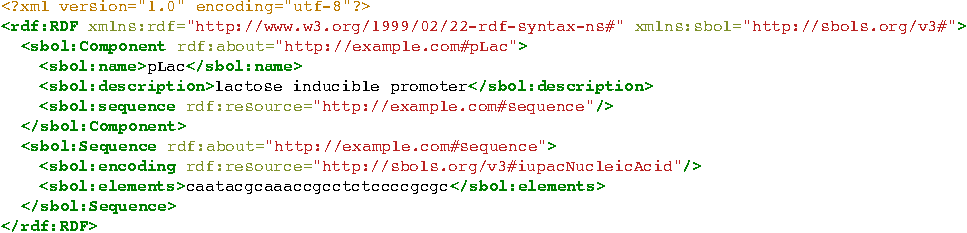
\includegraphics{example_serialization/example_rdfxml.pdf}

Alternatively, the same example can be serialized in Turtle as follows:

\vspace{3mm}
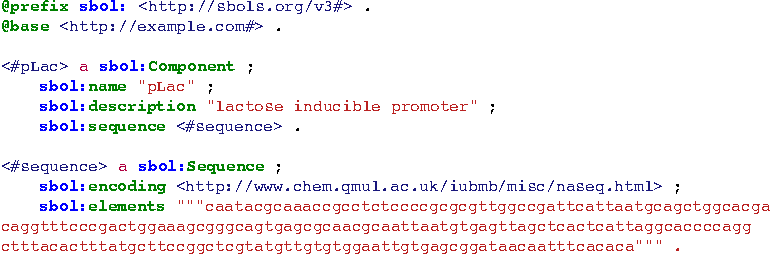
\includegraphics{example_serialization/example_turtle.pdf}

\threezeroone{\sbol{All SBOL libraries SHOULD support at least RDF/XML, N-Triples, JSON-LD, and Turtle.
Other SBOL tools SHOULD support at least one of these four formats.}}
